\documentclass[12pt,aspectratio=1610]{ecnubeamerformyself}

% Override image paths (set here so the .cls keeps defaults)
% \renewcommand{\ECNUBackgroundImage}{img/bg.pdf}
% \renewcommand{\ECNUFrameLogoImage}{img/logo-white.pdf}
% \renewcommand{\ECNUFirstPageBG}{img/firstpagebg.jpg}
% \renewcommand{\ECNUMathLogo}{img/math-logo.pdf}
% \renewcommand{\ECNULibThanks}{img/lib.png}

\addbibresource{../ref.bib}
%一些常用的宏定义
\newcommand{\bbA}{{\mathbb{A}}}
\newcommand{\bba}{{\mathbb{a}}}
\newcommand{\bbB}{{\mathbb{B}}}
\newcommand{\bbb}{{\mathbb{b}}}
\newcommand{\bbC}{{\mathbb{C}}}
\newcommand{\bbc}{{\mathbb{c}}}
\newcommand{\bbD}{{\mathbb{D}}} 
\newcommand{\bbd}{{\mathbb{d}}}
\newcommand{\bbE}{{\mathbb{E}}}
\newcommand{\bbe}{{\mathbb{e}}}
\newcommand{\bbF}{{\mathbb{F}}}
\newcommand{\bbf}{{\mathbb{f}}}
\newcommand{\bbG}{{\mathbb{G}}}
\newcommand{\bbg}{{\mathbb{g}}}
\newcommand{\bbH}{{\mathbb{H}}}
\newcommand{\bbh}{{\mathbb{h}}}
\newcommand{\bbI}{{\mathbb{I}}}
\newcommand{\bbi}{{\mathbb{i}}}
\newcommand{\bbJ}{{\mathbb{J}}}
\newcommand{\bbj}{{\mathbb{j}}}
\newcommand{\bbK}{{\mathbb{K}}}
\newcommand{\bbk}{{\mathbb{k}}}
\newcommand{\bbL}{{\mathbb{L}}}
\newcommand{\bbl}{{\mathbb{l}}}
\newcommand{\bbM}{{\mathbb{M}}}
\newcommand{\bbm}{{\mathbb{m}}}
\newcommand{\bbN}{{\mathbb{N}}}
\newcommand{\bbn}{{\mathbb{n}}}
\newcommand{\bbO}{{\mathbb{O}}}
\newcommand{\bbo}{{\mathbb{o}}}
\newcommand{\bbP}{{\mathbb{P}}}
\newcommand{\bbp}{{\mathbb{p}}}
\newcommand{\bbQ}{{\mathbb{Q}}}
\newcommand{\bbq}{{\mathbb{q}}}
\newcommand{\bbR}{{\mathbb{R}}}
\newcommand{\bbr}{{\mathbb{r}}}
\newcommand{\bbS}{{\mathbb{S}}}
\newcommand{\bbs}{{\mathbb{s}}}
\newcommand{\bbT}{{\mathbb{T}}}
\newcommand{\bbt}{{\mathbb{t}}}
\newcommand{\bbU}{{\mathbb{U}}}
\newcommand{\bbu}{{\mathbb{u}}}
\newcommand{\bbV}{{\mathbb{V}}}
\newcommand{\bbv}{{\mathbb{v}}}
\newcommand{\bbW}{{\mathbb{W}}}
\newcommand{\bbw}{{\mathbb{w}}}
\newcommand{\bbX}{{\mathbb{X}}}
\newcommand{\bbx}{{\mathbb{x}}}
\newcommand{\bbY}{{\mathbb{Y}}}
\newcommand{\bby}{{\mathbb{y}}}
\newcommand{\bbZ}{{\mathbb{Z}}}
\newcommand{\bbz}{{\mathbb{z}}}
\newcommand{\bbone}{{\mathbb{1}}}

\newcommand{\calA}{{\mathcal{A}}}
\newcommand{\cala}{{\mathcal{a}}}
\newcommand{\calB}{{\mathcal{B}}}
\newcommand{\calb}{{\mathcal{b}}}
\newcommand{\calC}{{\mathcal{C}}}
\newcommand{\calc}{{\mathcal{c}}}
\newcommand{\calD}{{\mathcal{D}}}
\newcommand{\cald}{{\mathcal{d}}}
\newcommand{\calE}{{\mathcal{E}}}
\newcommand{\cale}{{\mathcal{e}}}
\newcommand{\calF}{{\mathcal{F}}}
\newcommand{\calf}{{\mathcal{f}}}
\newcommand{\calG}{{\mathcal{G}}}
\newcommand{\calg}{{\mathcal{g}}}
\newcommand{\calH}{{\mathcal{H}}}
\newcommand{\calh}{{\mathcal{h}}}
\newcommand{\calI}{{\mathcal{I}}}
\newcommand{\cali}{{\mathcal{i}}}
\newcommand{\calJ}{{\mathcal{J}}}
\newcommand{\calj}{{\mathcal{j}}}
\newcommand{\calK}{{\mathcal{K}}}
\newcommand{\calk}{{\mathcal{k}}}
\newcommand{\calL}{{\mathcal{L}}}
\newcommand{\call}{{\mathcal{l}}}
\newcommand{\calM}{{\mathcal{M}}}
\newcommand{\calm}{{\mathcal{m}}}
\newcommand{\calN}{{\mathcal{N}}}
\newcommand{\caln}{{\mathcal{n}}}
\newcommand{\calO}{{\mathcal{O}}}
\newcommand{\calo}{{\mathcal{o}}}
\newcommand{\calP}{{\mathcal{P}}}
\newcommand{\calp}{{\mathcal{p}}}
\newcommand{\calQ}{{\mathcal{Q}}}
\newcommand{\calq}{{\mathcal{q}}}
\newcommand{\calR}{{\mathcal{R}}}
\newcommand{\calr}{{\mathcal{r}}}
\newcommand{\calS}{{\mathcal{S}}}
\newcommand{\cals}{{\mathcal{s}}}
\newcommand{\calT}{{\mathcal{T}}}
\newcommand{\calt}{{\mathcal{t}}}
\newcommand{\calU}{{\mathcal{U}}}
\newcommand{\calu}{{\mathcal{u}}}
\newcommand{\calV}{{\mathcal{V}}}
\newcommand{\calv}{{\mathcal{v}}}
\newcommand{\calW}{{\mathcal{W}}}
\newcommand{\calw}{{\mathcal{w}}}
\newcommand{\calX}{{\mathcal{X}}}
\newcommand{\calx}{{\mathcal{x}}}
\newcommand{\calY}{{\mathcal{Y}}}
\newcommand{\caly}{{\mathcal{y}}}
\newcommand{\calZ}{{\mathcal{Z}}}
\newcommand{\calz}{{\mathcal{z}}}

\newcommand{\frakA}{{\mathfrak{A}}}
\newcommand{\fraka}{{\mathfrak{a}}}
\newcommand{\frakB}{{\mathfrak{B}}}
\newcommand{\frakb}{{\mathfrak{b}}}
\newcommand{\frakC}{{\mathfrak{C}}}
\newcommand{\frakc}{{\mathfrak{c}}}
\newcommand{\frakD}{{\mathfrak{D}}}
\newcommand{\frakd}{{\mathfrak{d}}}
\newcommand{\frakE}{{\mathfrak{E}}}
\newcommand{\frake}{{\mathfrak{e}}}
\newcommand{\frakF}{{\mathfrak{F}}}
\newcommand{\frakf}{{\mathfrak{f}}}
\newcommand{\frakG}{{\mathfrak{G}}}
\newcommand{\frakg}{{\mathfrak{g}}}
\newcommand{\frakH}{{\mathfrak{H}}}
\newcommand{\frakh}{{\mathfrak{h}}}
\newcommand{\frakI}{{\mathfrak{I}}}
\newcommand{\fraki}{{\mathfrak{i}}}
\newcommand{\frakJ}{{\mathfrak{J}}}
\newcommand{\frakj}{{\mathfrak{j}}}
\newcommand{\frakK}{{\mathfrak{K}}}
\newcommand{\frakk}{{\mathfrak{k}}}
\newcommand{\frakL}{{\mathfrak{L}}}
\newcommand{\frakl}{{\mathfrak{l}}}
\newcommand{\frakM}{{\mathfrak{M}}}
\newcommand{\frakm}{{\mathfrak{m}}}
\newcommand{\frakN}{{\mathfrak{N}}}
\newcommand{\frakn}{{\mathfrak{n}}}
\newcommand{\frakO}{{\mathfrak{O}}}
\newcommand{\frako}{{\mathfrak{o}}}
\newcommand{\frakP}{{\mathfrak{P}}}
\newcommand{\frakp}{{\mathfrak{p}}}
\newcommand{\frakQ}{{\mathfrak{Q}}}
\newcommand{\frakq}{{\mathfrak{q}}}
\newcommand{\frakR}{{\mathfrak{R}}}
\newcommand{\frakr}{{\mathfrak{r}}}
\newcommand{\frakS}{{\mathfrak{S}}}
\newcommand{\fraks}{{\mathfrak{s}}}
\newcommand{\frakT}{{\mathfrak{T}}}
\newcommand{\frakt}{{\mathfrak{t}}}
\newcommand{\frakU}{{\mathfrak{U}}}
\newcommand{\fraku}{{\mathfrak{u}}}
\newcommand{\frakV}{{\mathfrak{V}}}
\newcommand{\frakv}{{\mathfrak{v}}}
\newcommand{\frakW}{{\mathfrak{W}}}
\newcommand{\frakw}{{\mathfrak{w}}}
\newcommand{\frakX}{{\mathfrak{X}}}
\newcommand{\frakx}{{\mathfrak{x}}}
\newcommand{\frakY}{{\mathfrak{Y}}}
\newcommand{\fraky}{{\mathfrak{y}}}
\newcommand{\frakZ}{{\mathfrak{Z}}}
\newcommand{\frakz}{{\mathfrak{z}}}

\newcommand{\rmA}{{\mathrm{A}}}
\newcommand{\rma}{{\mathrm{a}}}
\newcommand{\rmB}{{\mathrm{B}}}
\newcommand{\rmb}{{\mathrm{b}}}
\newcommand{\rmC}{{\mathrm{C}}}
\newcommand{\rmc}{{\mathrm{c}}}
\newcommand{\rmD}{{\mathrm{D}}}
\newcommand{\rmd}{{\mathrm{d}}}
\newcommand{\rmE}{{\mathrm{E}}}
\newcommand{\rme}{{\mathrm{e}}}
\newcommand{\rmF}{{\mathrm{F}}}
\newcommand{\rmf}{{\mathrm{f}}}
\newcommand{\rmG}{{\mathrm{G}}}
\newcommand{\rmg}{{\mathrm{g}}}
\newcommand{\rmH}{{\mathrm{H}}}
\newcommand{\rmh}{{\mathrm{h}}}
\newcommand{\rmI}{{\mathrm{I}}}
\newcommand{\rmi}{{\mathrm{i}}}
\newcommand{\rmJ}{{\mathrm{J}}}
\newcommand{\rmj}{{\mathrm{j}}}
\newcommand{\rmK}{{\mathrm{K}}}
\newcommand{\rmk}{{\mathrm{k}}}
\newcommand{\rmL}{{\mathrm{L}}}
\newcommand{\rml}{{\mathrm{l}}}
\newcommand{\rmM}{{\mathrm{M}}}
\newcommand{\rmm}{{\mathrm{m}}}
\newcommand{\rmN}{{\mathrm{N}}}
\newcommand{\rmn}{{\mathrm{n}}}
\newcommand{\rmO}{{\mathrm{O}}}
\newcommand{\rmo}{{\mathrm{o}}}
\newcommand{\rmP}{{\mathrm{P}}}
\newcommand{\rmp}{{\mathrm{p}}}
\newcommand{\rmQ}{{\mathrm{Q}}}
\newcommand{\rmq}{{\mathrm{q}}}
\newcommand{\rmR}{{\mathrm{R}}}
\newcommand{\rmr}{{\mathrm{r}}}
\newcommand{\rmS}{{\mathrm{S}}}
\newcommand{\rms}{{\mathrm{s}}}
\newcommand{\rmT}{{\mathrm{T}}}
\newcommand{\rmt}{{\mathrm{t}}}
\newcommand{\rmU}{{\mathrm{U}}}
\newcommand{\rmu}{{\mathrm{u}}}
\newcommand{\rmV}{{\mathrm{V}}}
\newcommand{\rmv}{{\mathrm{v}}}
\newcommand{\rmW}{{\mathrm{W}}}
\newcommand{\rmw}{{\mathrm{w}}}
\newcommand{\rmX}{{\mathrm{X}}}
\newcommand{\rmx}{{\mathrm{x}}}
\newcommand{\rmY}{{\mathrm{Y}}}
\newcommand{\rmy}{{\mathrm{y}}}
\newcommand{\rmZ}{{\mathrm{Z}}}

\newcommand{\bfA}{{\mathbf{A}}}
\newcommand{\bfa}{{\mathbf{a}}}
\newcommand{\bfB}{{\mathbf{B}}}
\newcommand{\bfb}{{\mathbf{b}}}
\newcommand{\bfC}{{\mathbf{C}}}
\newcommand{\bfc}{{\mathbf{c}}}
\newcommand{\bfD}{{\mathbf{D}}}
\newcommand{\bfd}{{\mathbf{d}}}
\newcommand{\bfE}{{\mathbf{E}}}
\newcommand{\bfe}{{\mathbf{e}}}
\newcommand{\bfF}{{\mathbf{F}}}
\newcommand{\bff}{{\mathbf{f}}}
\newcommand{\bfG}{{\mathbf{G}}}
\newcommand{\bfg}{{\mathbf{g}}}
\newcommand{\bfH}{{\mathbf{H}}}
\newcommand{\bfh}{{\mathbf{h}}}
\newcommand{\bfI}{{\mathbf{I}}}
\newcommand{\bfi}{{\mathbf{i}}}
\newcommand{\bfJ}{{\mathbf{J}}}
\newcommand{\bfj}{{\mathbf{j}}}
\newcommand{\bfK}{{\mathbf{K}}}
\newcommand{\bfk}{{\mathbf{k}}}
\newcommand{\bfL}{{\mathbf{L}}}
\newcommand{\bfl}{{\mathbf{l}}}
\newcommand{\bfM}{{\mathbf{M}}}
\newcommand{\bfm}{{\mathbf{m}}}
\newcommand{\bfN}{{\mathbf{N}}}
\newcommand{\bfn}{{\mathbf{n}}}
\newcommand{\bfO}{{\mathbf{O}}}
\newcommand{\bfo}{{\mathbf{o}}}
\newcommand{\bfP}{{\mathbf{P}}}
\newcommand{\bfp}{{\mathbf{p}}}
\newcommand{\bfQ}{{\mathbf{Q}}}
\newcommand{\bfq}{{\mathbf{q}}}
\newcommand{\bfR}{{\mathbf{R}}}
\newcommand{\bfr}{{\mathbf{r}}}
\newcommand{\bfS}{{\mathbf{S}}}
\newcommand{\bfs}{{\mathbf{s}}}
\newcommand{\bfT}{{\mathbf{T}}}
\newcommand{\bft}{{\mathbf{t}}}
\newcommand{\bfU}{{\mathbf{U}}}
\newcommand{\bfu}{{\mathbf{u}}}
\newcommand{\bfV}{{\mathbf{V}}}
\newcommand{\bfv}{{\mathbf{v}}}
\newcommand{\bfW}{{\mathbf{W}}}
\newcommand{\bfw}{{\mathbf{w}}}
\newcommand{\bfX}{{\mathbf{X}}}
\newcommand{\bfx}{{\mathbf{x}}}
\newcommand{\bfY}{{\mathbf{Y}}}
\newcommand{\bfy}{{\mathbf{y}}}
\newcommand{\bfZ}{{\mathbf{Z}}}
\newcommand{\bfz}{{\mathbf{z}}}

\newcommand{\sfA}{{\mathsf{A}}}
\newcommand{\sfa}{{\mathsf{a}}}
\newcommand{\sfB}{{\mathsf{B}}}
\newcommand{\sfb}{{\mathsf{b}}}
\newcommand{\sfC}{{\mathsf{C}}}
\newcommand{\sfc}{{\mathsf{c}}}
\newcommand{\sfD}{{\mathsf{D}}}
\newcommand{\sfd}{{\mathsf{d}}}
\newcommand{\sfE}{{\mathsf{E}}}
\newcommand{\sfe}{{\mathsf{e}}}
\newcommand{\sfF}{{\mathsf{F}}}
\newcommand{\sff}{{\mathsf{f}}}
\newcommand{\sfG}{{\mathsf{G}}}
\newcommand{\sfg}{{\mathsf{g}}}
\newcommand{\sfH}{{\mathsf{H}}}
\newcommand{\sfh}{{\mathsf{h}}}
\newcommand{\sfI}{{\mathsf{I}}}
\newcommand{\sfi}{{\mathsf{i}}}
\newcommand{\sfJ}{{\mathsf{J}}}
\newcommand{\sfj}{{\mathsf{j}}}
\newcommand{\sfK}{{\mathsf{K}}}
\newcommand{\sfk}{{\mathsf{k}}}
\newcommand{\sfL}{{\mathsf{L}}}
\newcommand{\sfl}{{\mathsf{l}}}
\newcommand{\sfM}{{\mathsf{M}}}
\newcommand{\sfm}{{\mathsf{m}}}
\newcommand{\sfN}{{\mathsf{N}}}
\newcommand{\sfn}{{\mathsf{n}}}
\newcommand{\sfO}{{\mathsf{O}}}
\newcommand{\sfo}{{\mathsf{o}}}
\newcommand{\sfP}{{\mathsf{P}}}
\newcommand{\sfp}{{\mathsf{p}}}
\newcommand{\sfQ}{{\mathsf{Q}}}
\newcommand{\sfq}{{\mathsf{q}}}
\newcommand{\sfR}{{\mathsf{R}}}
\newcommand{\sfr}{{\mathsf{r}}}
\newcommand{\sfS}{{\mathsf{S}}}
\newcommand{\sfs}{{\mathsf{s}}}
\newcommand{\sfT}{{\mathsf{T}}}
\newcommand{\sft}{{\mathsf{t}}}
\newcommand{\sfU}{{\mathsf{U}}}
\newcommand{\sfu}{{\mathsf{u}}}
\newcommand{\sfV}{{\mathsf{V}}}
\newcommand{\sfv}{{\mathsf{v}}}
\newcommand{\sfW}{{\mathsf{W}}}
\newcommand{\sfw}{{\mathsf{w}}}
\newcommand{\sfX}{{\mathsf{X}}}
\newcommand{\sfx}{{\mathsf{x}}}
\newcommand{\sfY}{{\mathsf{Y}}}
\newcommand{\sfy}{{\mathsf{y}}}
\newcommand{\sfZ}{{\mathsf{Z}}}
\newcommand{\sfz}{{\mathsf{z}}}


\newcommand{\kk}{{\mathbf{k}}}
\newcommand{\kkk}{{\mathbb{k}}}
\newcommand{\KK}{{\mathbf{K}}}
\newcommand{\KKK}{{\mathbb{K}}}
\newcommand{\rkk}{{\kappa}} % residue field
\newcommand{\fkk}{{\mathscr{K}}} % fraction field

\renewcommand{\d}{{\mathrm{d}}}
\renewcommand{\i}{{\mathrm{i}}}
\renewcommand{\P}{\partial}


\newcommand{\Set}{\mathbf{Set}}
\newcommand{\Var}{\mathbf{Var}}
\newcommand{\Sch}{\mathbf{Sch}}
\newcommand{\Alg}{\mathbf{Alg}}
\newcommand{\Ring}{\mathbf{Ring}}
\newcommand{\Mod}{\mathbf{Mod}}
\newcommand{\TopMod}{\mathbf{TopMod}}
\newcommand{\Grp}{\mathbf{Grp}}
\newcommand{\Ab}{\mathbf{Ab}}
\newcommand{\Top}{\mathbf{Top}}
\newcommand{\Cat}{\mathbf{Cat}}
\newcommand{\AlgSp}{\mathbf{AlgSp}}
\newcommand{\Obj}{\operatorname{Obj}}


\newcommand{\ten}{\otimes}
\newcommand{\ratmap}{\dasharrow}
\newcommand{\injmap}{\hookrightarrow}
\newcommand{\surjmap}{\twoheadrightarrow}

\newcommand{\id}{{\operatorname{id}}}

\newcommand{\Frac}{\operatorname{Frac}}
\newcommand{\Der}{\operatorname{Der}}
\newcommand{\Spec}{\operatorname{Spec}}
\newcommand{\spec}{\operatorname{Spec}}
\newcommand{\mSpec}{\operatorname{mSpec}}
\newcommand{\depth}{\operatorname{depth}}
\newcommand{\idealht}{\operatorname{ht}}
\newcommand{\codim}{\operatorname{codim}}
\newcommand{\Supp}{\operatorname{Supp}}
\newcommand{\trdeg}{\operatorname{trdeg}}
\newcommand{\Ass}{\operatorname{Ass}}
\newcommand{\Ann}{\operatorname{Ann}}
\newcommand{\Ext}{\operatorname{Ext}}
\newcommand{\Tor}{\operatorname{Tor}}
\newcommand{\Hom}{\operatorname{Hom}}
\newcommand{\Eq}{\operatorname{Eq}}
\newcommand{\End}{\operatorname{End}}
\newcommand{\Mor}{\operatorname{Mor}}
\newcommand{\Mult}{\operatorname{Mult}}
\renewcommand{\Im}{\operatorname{Im}}
\newcommand{\Ker}{\operatorname{Ker}}
\newcommand{\rank}{\operatorname{rank}}
\newcommand{\cohdim}{\operatorname{coh.dim}}
\newcommand{\hldim}{\operatorname{hl.dim}}
\newcommand{\projdim}{\operatorname{proj.dim}}
\newcommand{\injdim}{\operatorname{inj.dim}}
\newcommand{\rad}{\operatorname{rad}}
\newcommand{\nil}{\operatorname{nil}}
\newcommand{\characteristic}{\operatorname{char}}
\newcommand{\Pic}{\operatorname{Pic}}
\newcommand{\NS}{\operatorname{NS}}
\newcommand{\Exc}{\operatorname{Exc}}
\newcommand{\Sing}{\operatorname{Sing}}
\newcommand{\Reg}{\operatorname{Reg}}
\newcommand{\Tr}{\operatorname{Tr}}
\newcommand{\Psef}{\operatorname{Psef}}
\newcommand{\Nef}{\operatorname{Nef}}
\newcommand{\Amp}{\operatorname{Amp}}
\newcommand{\Bigcone}{\operatorname{Big}}
\newcommand{\Frob}{\operatorname{Frob}}
\newcommand{\Bs}{\operatorname{Bs}}
\newcommand{\Stab}{\operatorname{Stab}}
\newcommand{\Sp}{\operatorname{Sp}}


\newcommand{\calHom}{{\mathcal{H\!o\!m}}}
\newcommand{\calExt}{{\mathcal{Ext}}}
\newcommand{\calProj}{{\mathcal{P\!r\!o\!j}}}
\newcommand{\calSpec}{{\mathcal{S\!p\!e\!c}}}


\newcommand{\mat}[4]{\left[ \begin{array}{cc}#1 &#2 \\ #3 &#4\end{array}\right]}
\newcommand{\threemat}[9]{\left[ \begin{array}{ccc}
  #1 & #2 & #3 \\
  #4 & #5 & #6 \\
  #7 & #8 & #9
\end{array}\right]}
\newcommand{\genmat}[9]{\left( \begin{array}{cccc}
  #1 & #2 & \cdots & #3 \\
  #4 & #5 & \cdots & #6 \\  
  \ldots & \ldots & \ddots & \ldots \\
  #7 & #8 & \cdots & #9
\end{array}\right)}





\newcommand{\contradiction}{
    \raisebox{-0.6ex}{\makebox[2.4ex][c]{
\begin{tikzpicture}
        \draw (0,0) circle (1.2ex);
        \draw (0.7 ex, 0.7 ex) -- (-0.4 ex, 0.7 ex);
        \draw (-0.4 ex, 0.7 ex) -- (0.7 ex, -0.4 ex);
        \draw (0.7 ex, -0.4 ex) -- (0.7 ex, 0.7 ex);
        \draw (0.7 ex, 0.7 ex) -- (-0.848 ex, -0.848 ex);
    \end{tikzpicture}}}
    \ \ 
}

% legendre符号
\makeatletter
\def\legendre@dash#1#2{\hb@xt@#1{%
  \kern-#2\p@
  \cleaders\hbox{\kern.5\p@
    \vrule\@height.2\p@\@depth.2\p@\@width\p@
    \kern.5\p@}\hfil
  \kern-#2\p@
  }}
\def\@legendre#1#2#3#4#5{\mathopen{}\left(
  \sbox\z@{$\genfrac{}{}{0pt}{#1}{#3#4}{#3#5}$}%
  \dimen@=\wd\z@
  \kern-\p@\vcenter{\box0}\kern-\dimen@\vcenter{\legendre@dash\dimen@{#2}}\kern-\p@
  \right)\mathclose{}}
\newcommand\legendre[2]{\mathchoice
  {\@legendre{0}{1}{}{#1}{#2}}
  {\@legendre{1}{.5}{\vphantom{1}}{#1}{#2}}
  {\@legendre{2}{0}{\vphantom{1}}{#1}{#2}}
  {\@legendre{3}{0}{\vphantom{1}}{#1}{#2}}
}
\def\dlegendre{\@legendre{0}{1}{}}
\def\tlegendre{\@legendre{1}{0.5}{\vphantom{1}}}
\makeatother
\usetikzlibrary{arrows.meta,calc}

\def\acts{\ \rotatebox[origin=c]{-90}{$\circlearrowright$}\ }
\def\racts{\ \rotatebox[origin=c]{90}{$\circlearrowleft$}\ }
% \def\dacts{\ \rotatebox[origin=c]{0}{$\circlearrowright$}\ }
% \def\uacts{\ \rotatebox[origin=c]{180}{$\circlearrowright$}\ }

\title{Algebraic Dynamics and Dynamical Iitaka Theory}
% \subtitle{}
\date{ICCM 2025, January 7, 2026}
\author{Tianle Yang \texorpdfstring{\\}{,} based on the joint work with Sheng Meng and Long Wang}


% Institute logo on the title page
\titlegraphic{\hfill\includegraphics[height=1.2cm]{\ECNUMathLogo}}


\begin{document}

% First page with different background
{
    \setbeamertemplate{background}{
        \includegraphics[width=\paperwidth,height=\paperheight]{\ECNUFirstPageBG}
    }
    \maketitle
}


% ----------------------------------------------------------


\begin{frame}{Kawaguchi-Silverman Conjecture}

    Work over \(\overline{\bbQ}\).
    \(X\): smooth projective variety,
    \(f:X \to X\): surjective endomorphism.
    \(H\): ample divisor on \(X\).
    \(h:X(\overline{\bbQ}) \to \bbR_{\geq 1}\): a height function associated to \(H\).
        
    \begin{conjecture}[{Kawaguchi-Silverman Conjecture $=$ KSC}]\label{conj: ksc} 
        If the orbit \(O_f(x):=\{f^n(x)\,|\,n\ge 0\}\) is Zariski dense in \(X\), then
        \[ \alpha_f(x) = \delta_f.  \]
    \end{conjecture} 

    here,
    \[
        \alpha_f(x) := \lim_{n\to\infty} h(f^n(x))^{1/n},
    \]
    arithmetic invariant at \(x\),
    \[
        \delta_f := \lim_{n\to\infty} ((f^n)^*H \cdot H^{\dim X - 1})^{1/n},
    \]
    geometric invariant of \(f\).
    
\end{frame}


\begin{frame}{An example}
    \vskip-1em
    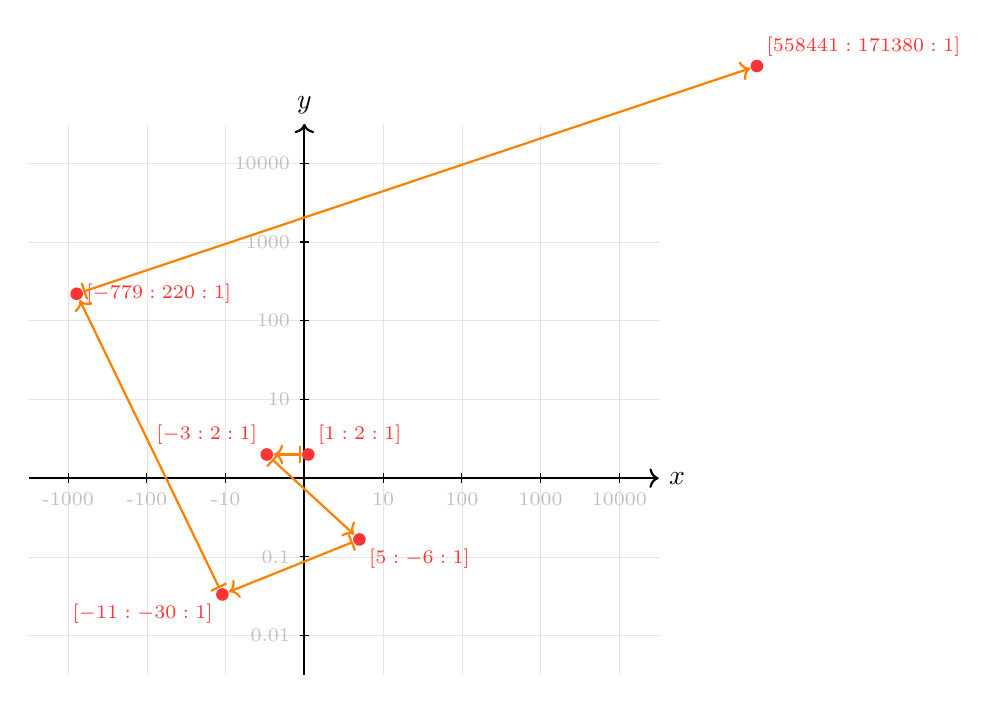
\begin{tikzpicture}
        % axes from -4 to 4 with grid and ticks
        \draw[help lines, gray!20] (-3.5,-2.5) grid (4.5,4.5);
        \draw[->, thick] (-3.5,0) -- (4.5,0) node[right] {$x$};
        \draw[->, thick] (0,-2.5) -- (0,4.5) node[above] {$y$};
        \foreach \pos/\labels in {-3/{-1000}, -2/{-100}, -1/{-10}, 1/{10}, 2/{100}, 3/{1000}, 4/{10000}}{
            \draw (\pos,0.06) -- (\pos,-0.06) node[below,text=gray!50,font=\scriptsize] {\labels};
        }
        \foreach \pos/\labels in {-2/{0.01}, -1/{0.1}, 1/{10}, 2/{100}, 3/{1000}, 4/{10000}}{
            \draw (0.06,\pos) -- (-0.06,\pos) node[left,text=gray!50,font=\scriptsize] {\labels};
        }

        % draw the orbit points and arrows between them
        
        % define named coordinates for the orbit points
        \coordinate (p0) at (0.05,0.301);
        \coordinate (p1) at (-0.477,0.301);
        \coordinate (p2) at (0.699,-0.778);
        \coordinate (p3) at (-1.041,-1.477);
        \coordinate (p4) at (-2.892,2.342);
        \coordinate (p5) at (5.747,5.234);

        % draw the filled points
        \foreach \p in {p0,p1,p2,p3,p4,p5}{
            \fill[red!80] (\p) circle (0.08);
        }

        % draw labels for the points
        \node[above right,font=\scriptsize,text=red!80] at (p0) {\([1:2:1]\)};
        \node[above left,font=\scriptsize,text=red!80] at (p1) {\([-3:2:1]\)};
        \node[below right,font=\scriptsize,text=red!80] at (p2) {\([5:-6:1]\)};
        \node[below left,font=\scriptsize,text=red!80] at (p3) {\([-11:-30:1]\)};
        \node[right,font=\scriptsize,text=red!80] at (p4) {\([-779:220:1]\)};
        \node[above right,font=\scriptsize,text=red!80] at (p5) {\([558441:171380:1]\)};

        % draw arrows between named points
        \draw[|->,thick,orange,shorten <=0.09cm,shorten >=0.09cm] (p0) -- (p1);
        \draw[|->,thick,orange,shorten <=0.09cm,shorten >=0.09cm] (p1) -- (p2);
        \draw[|->,thick,orange,shorten <=0.09cm,shorten >=0.09cm] (p2) -- (p3);
        \draw[|->,thick,orange,shorten <=0.09cm,shorten >=0.09cm] (p3) -- (p4);
        \draw[|->,thick,orange,shorten <=0.09cm,shorten >=0.09cm] (p4) -- (p5);

    \end{tikzpicture}

    \begin{tikzpicture}[remember picture,overlay]
    \node[anchor=south east,xshift=-0.6cm,yshift=0.8cm] at (current page.south east) {%
        \begin{minipage}[c][8cm]{0.44\textwidth}
            {\fontsize{9pt}{11pt}\selectfont
                \setbeamertemplate{itemize item}{\Large\textbullet}
                \begin{itemize}[<+- | alert@+>]
                    \setlength{\itemsep}{8pt}
                    \setlength{\parskip}{2pt}
                    \item 
                    \(X=\mathbb{P}^2\), 
                    
                    \(f:[x:y:z]\mapsto[x^2-y^2:xy:z^2]\),
                    
                    \(x = [1:2:1]\).

                    \item \(f^*H \sim 2H\) \(\Rightarrow\) \((f^n)^*H \sim 2^n H\) \(\Rightarrow\) \(\delta_f = 2\).
                    
                    \item 
                    \begin{tabular}{r l l}
                    \(n\) & \(h(f^n(x))\)   &   \\ \hline
                    \(0\) & \(\log 2\)      & \approx \(0.7\) \\
                    \(1\) & \(\log 3\)      & \approx \(1.1\) \\
                    \(2\) & \(\log 6\)      & \approx \(1.8\) \\
                    \(3\) & \(\log 30\)     & \approx \(3.4\) \\
                    \(4\) & \(\log 779\)    & \approx \(6.7\) \\
                    \(5\) & \(\log 558441\) & \approx \(13.2\)
                    \end{tabular}

                    \item It is expected that \(\alpha_f(x) = 2\).

                \end{itemize}
            }
        \end{minipage}
    };
    \end{tikzpicture}

    % Let \(X=\mathbb{P}^2\) and \(f:[x:y:z]\mapsto[x^2-y^2:xy:z^2]\).

    % \(x=[1:2:1]\) has a Zariski dense orbit and \(\delta_f=2\).
    % \(f(x)=[-3:2:1]\), 
    % \(f^2(x)=[5:-6:1]\), 
    % \(f^3(x)=[-11:-30:1]\), 
    % \(f^4(x)=[-779:220:1]\), 
    % \(f^5(x)=[558441:171380:1]\), 

    % log10 coordinates of the orbit points:
    % \((0,0.301),(-0.477,0.301),(0.699,-0.778),(-1.041,-1.477),(-2.892,2.342),(5.747,5.234),\ldots\)

    % Heights:
    % \(h(x)=\log\max\{|1|,|2|,|1|\}=\log2\approx0.7\),
    % \(h(f(x))=\log3\approx1.1\),
    % \(h(f^2(x))=\log6\approx1.8\),
    % \(h(f^3(x))=\log30\approx3.4\),
    % \(h(f^4(x))=\log779\approx6.7\),
    % \(h(f^5(x))=\log558441\approx13.2,\ldots\)
\end{frame}


\begin{frame}[c]{Three orbit conjectures}

    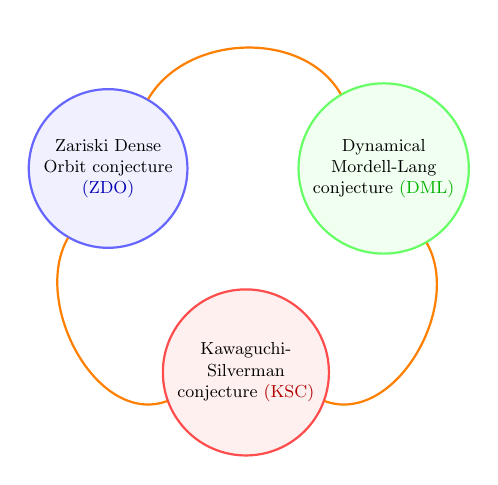
\begin{tikzpicture}[>=Stealth, every node/.style={font=\small}, scale=0.7, transform shape]
        % nodes
        \node[draw=blue!60, fill=blue!6, thick, circle, minimum size=2.5cm, align=center] (ZDO) at (-2.5,0) {Zariski Dense\\ Orbit conjecture\\ \textcolor{blue!70!black}{(ZDO)}};
        \node[draw=green!60, fill=green!6, thick, circle, minimum size=2.5cm, align=center] (DML) at (2.5,0) {Dynamical\\ Mordell-Lang\\ conjecture \textcolor{green!70!black}{(DML)}};
        \node[draw=red!70, fill=red!6, thick, circle, minimum size=2.5cm, align=center] (KSC) at (0,-3.7) {Kawaguchi-\\Silverman\\ conjecture \textcolor{red!70!black}{(KSC)}};

        % curved association arrows
        \draw[-, thick, orange] (ZDO) to[out=60,in=120] (DML);
        \draw[-, thick, orange] (DML) to[out=-60,in=-20] (KSC);
        \draw[-, thick, orange] (KSC) to[out=-160,in=-120] (ZDO);
    \end{tikzpicture}

    \begin{tikzpicture}[remember picture,overlay]
    \node[anchor=east,xshift=-0.6cm] at (current page.east) {%
        \begin{minipage}[t][0.9\textheight]{0.55\textwidth}
            \only<1-3>{
                \textcolor{red!70!black}{
                    The KSC relates the growth rate of heights along orbits to dynamical degrees.
                }
            }

            \only<2-3>{
                \vspace{0.3cm}
                \textcolor{green!70!black}{
                    The DML predicts if 
                    \[ \# O_f(x) \cap V = \infty, \]
                    then 
                    \[ O_g(y) \subseteq V \]
                    for some \(y=f^r(x), g = f^s\).
                }
            }

            \only<3>{
                \vspace{0.3cm}
                \textcolor{blue!70!black}{
                    The ZDO states that either 
                    \[ \exists x\  \text{with}\  \overline{O_f(x)} = X, \]
                    or 
                    \[ \exists\  f^n \acts X \ratmap Y \racts \id_Y. \]
                }
            }

            \only<4->{Main known cases:}

            \only<5>{
                \vspace{0.3cm}
                \textcolor{red!70!black}{
                    Endomorphisms of projective surfaces [Matsuzawa-Sano-Shibata];\\
                    Birational map of projective surfaces [Wang, to be checked];\\
                    Int-amplified endomorphisms [Meng-Zhong];\\
                    Non-isomorphic surjective endomorphism on threefolds [Meng-Zhang];\\
                }
            }

            \only<6-7>{
                \vspace{0.3cm}
                \textcolor{green!70!black}{
                    DML in the \'etale case [Bell-Ghioca-Tucker] ;\\
                    DML for endomorphisms of \(\bbA^2\) [Xie];\\
                }
            }

            \only<7>{
                \vspace{0.3cm}
                \textcolor{blue!70!black}{
                    The ZDO for endomorphisms of surfaces [Xie,Jia-Xie-Zhang];\\
                    The ZDO for automorphisms of threefolds with positive entropy [Matsuzawa-Xie]
                }
            }
        \end{minipage}
    };
    \end{tikzpicture}
    
\end{frame}


\begin{frame}[c]{Dynamical Iitaka Theory}

    \begin{columns}[c]  
        \begin{column}{0.4\textwidth}
            Coarse classification of varieties via Kodaira dimension \(\kappa(X,K_X)\):
        \end{column}

        \begin{column}{0.6\textwidth}
            \centering
            \begin{tabular}{c|c}
                \hline
                $\kappa(X,K_X)$         & Typical geometry  \\
                \hline
                $-\infty$               & uniruled          \\
                $0$                     & Calabi-Yau        \\
                $0<\kappa(X)<\dim X$    & fibrations type   \\
                $\dim X$                & general type      \\
                \hline
            \end{tabular}
        \end{column}
    \end{columns}

    \pause
    \vspace{0.6cm}

    \begin{columns}[c]
        \begin{column}{0.4\textwidth}
            Dynamical analogue: classify \((X,f)\) via \(\kappa_f(X,R_f)\).
        \end{column}

        \begin{column}{0.6\textwidth}
            \centering
            \begin{tabular}{c|c}
                \hline
                $\kappa_f(X,R_f)$               & Typical dynamics                      \\
                \hline
                $0$                             & \(f\) is log-\'etale                  \\
                $0<\kappa_f(X,R_f)<\dim X$      & fibrations type                       \\
                $\dim X$                        & \(R_{f^s}\) is big for \(s \geq 0\)   \\
                \hline
            \end{tabular}
        \end{column}
    \end{columns}

\end{frame}


\begin{frame}{Main results}

    \only<1->{
        Settings:
        \begin{itemize}
            \item \(\pi:(X,f) \to (Y,g)\) smooth Fano fibration with \(X,Y\) smooth projective and \(\rho(X) = \rho(Y)+1\);
            \item \(Y\) is an abelian variety or of picard number one;
            \only<4->{\item \(f\) has a Zariski dense orbit;}
            \only<4->{\item \(\delta_f > \delta_g\);}
            \only<4->{\item if \(Y\) is of picard number one, then \(\delta_g = 1\).}
        \end{itemize}
    }

    \only<2-3>{
        \begin{theorem}[{[Meng-Wang-Y]}]\label{thm: mainthm}
            KSC holds for \((X,f)\) under the above settings.
        \end{theorem}
    }

    \only<2>{
        \vspace{0.5em}
        Generalize the following known results:
        \begin{itemize}
            \item 
        \end{itemize}
    }

    \only<3>{
        Sketch of idea:
        If \(\delta_f = \delta_g\), then 
        \vspace{0.5em}
        \[ \text{\shortstack{KSC for abelian varieties\\ or polarized endomorphisms}} \Rightarrow \text{KSC for } (Y,g) \Rightarrow \text{KSC for } (X,f). \]

        If \(\delta_f > \delta_g\), under some extra conditions, we have another fibration by dynamical Iitaka theory.
    }

    \only<4>{
        \begin{theorem}[{[Meng-Wang-Y]}]\label{thm: mainthm2}
            There is equivariant fibrations
            \[ f \acts X \overset{\varphi_{f,R_f}}{---\!\twoheadrightarrow} Y \racts g \]
            with \(\dim Y>0\) and \(g\) is \(q\)-polarized.
        \end{theorem}
    }
\end{frame}


\begin{frame}{Main results}

    \vspace{0.5em}

    \begin{theorem}[{[Meng-Zhang]}]
        \vspace{1em}
        Suppose that \(f^*R_f \equiv q R_f\) for some \(q > 1\).
        Then there exists an \(f\)-equivariant fibration (dynamical Iitaka fibration associated to \(R_f\))
        \[ f \acts X \overset{\varphi_{f,R_f}}{---\!\twoheadrightarrow} Y \racts g \]
        with \(\dim Y = \kappa_f(X,R_f)\) and \(g\) is \(q\)-polarized.
    \end{theorem}

    With help of this result, we only need to show that under our settings,

    \begin{itemize}
        \item \(\kappa_f(X,R_f) \geq 1\); \only<2->{ \(\Longleftarrow\) criterion for toric bundles}
        \item \(f^*R_f \equiv \delta_f R_f\). \only<3>{ \(\Longleftarrow\) decomposition of cones \(+\) no rational curve on \(Y\)}
    \end{itemize}

    Then 
    \[ \text{KSC for polarized endomorphisms} \implies \text{KSC for } (Y,g) \implies \text{KSC for } (X,f). \]

\end{frame}


\begin{frame}{Technique: decomposition of cones}

    \vspace{0.5em}

    \begin{theorem}[{[Meng-Wang-Y]}]\label{thm: cone-decomp}
        \vspace{0.5em}
        \begin{columns}[c]
            \begin{column}{0.4\textwidth}
                \centering
                \(\pi:(X,f) \to (Y,g)\) flat; \\
                \(X,Y\) smooth projective; \\
                \(\delta_f > \delta_g\);\(\rho(X) = \rho(Y)+1\).
            \end{column}

            \begin{column}{0.1\textwidth}
                \centering
                \[ \Longrightarrow \]
            \end{column}

            \begin{column}{0.5\textwidth}
                \centering
                \(\exists D\) nef with \(f^*D \equiv \delta_f D\) s.t.
                \[ \Psef^1(X) = \pi^*\Psef^1(Y) \oplus \bbR_{\geq 0} D,\] 
                \[ \Nef^1(X) = \pi^*\Nef^1(Y) \oplus \bbR_{\geq 0} D. \]
            \end{column}
        \end{columns}
    \end{theorem}

    \pause

    \begin{columns}[c]  
        \begin{column}{0.5\textwidth}
            \centering

            Cones of a general fibration \(\pi:X\to Y\):

            \vspace{1em}
            
            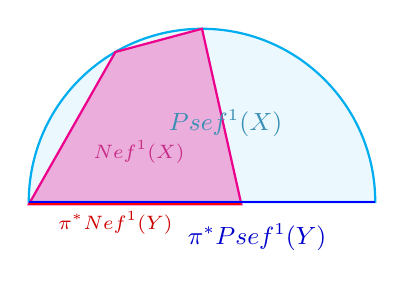
\begin{tikzpicture}[scale=1, every node/.style={font=\small}]
                % parameters
                \def\rrrr{2.2}
                \def\dddd{0.5}

                % semicircle (Psef^1(X))
                \fill[cyan!8,draw=cyan,thick] (-\rrrr,0) arc (180:0:\rrrr) -- cycle;
                % quadrangle (Nef^1(X))
                \fill[magenta, fill opacity=0.3, draw=magenta, thick] (-\rrrr,-0.03) -- (-0.5*\rrrr,0.866*\rrrr) -- (0,\rrrr) -- (\dddd,-0.03) -- cycle;
                \node[below,magenta!80!black,font=\scriptsize] at (-0.8,0.9) {\(\Nef^1(X)\)};
                % overall label for the semicircle
                \node[above,cyan!70!black] at (0.3,0.7) {\(\Psef^1(X)\)};

                % diameter line segment (Psef^1(Y)) (Nef^1(Y))
                \draw[thick,blue] (-\rrrr,0) -- (\rrrr,0);
                \node[below,blue!80!black] at (0.7,-0.15) {\(\pi^*\Psef^1(Y)\)};
                \draw[thick,red] (-\rrrr,-0.03) -- (\dddd,-0.03);
                \node[below,red!80!black,font=\scriptsize] at (-1.1,0) {\(\pi^*\Nef^1(Y)\)};
                
            \end{tikzpicture}
        \end{column}

        \pause

        \begin{column}{0.5\textwidth}
            \centering

            Cones of fibration with dynamical restrictions:

            \vspace{0.5em}

            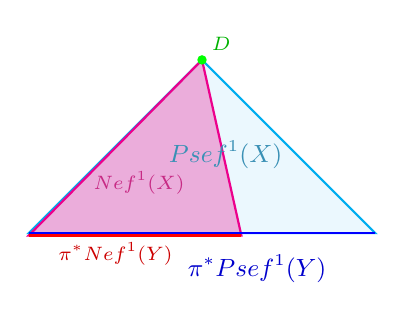
\begin{tikzpicture}[scale=1, every node/.style={font=\small}]
                % parameters
                \def\rrrr{2.2}
                \def\dddd{0.5}

                % triangle (Psef^1(X))
                \fill[cyan!8,draw=cyan,thick] (-\rrrr,0) -- (0,\rrrr) -- (\rrrr,0) -- cycle;
                % triangle (Nef^1(X))
                \fill[magenta, fill opacity=0.3, draw=magenta, thick] (-\rrrr,-0.03) -- (0,\rrrr) -- (\dddd,-0.03) -- cycle;
                \node[below,magenta!80!black,font=\scriptsize] at (-0.8,0.9) {\(\Nef^1(X)\)};
                % overall label for the semicircle
                \node[above,cyan!70!black] at (0.3,0.7) {\(\Psef^1(X)\)};

                % diameter line segment (Psef^1(Y)) (Nef^1(Y))
                \draw[thick,blue] (-\rrrr,0) -- (\rrrr,0);
                \node[below,blue!80!black] at (0.7,-0.15) {\(\pi^*\Psef^1(Y)\)};
                \draw[thick,red] (-\rrrr,-0.03) -- (\dddd,-0.03);
                \node[below,red!80!black,font=\scriptsize] at (-1.1,0) {\(\pi^*\Nef^1(Y)\)};

                % dot and label at (0,\rrrr)
                \fill[green] (0,\rrrr) circle (0.06);
                \node[above right,font=\scriptsize,green!70!black] at (0,\rrrr) {\(D\) };
            \end{tikzpicture}
        \end{column}
    \end{columns}
\end{frame}


\begin{frame}{Technique: criterion for toric bundles}
    \vspace{0.5em}
    \begin{theorem}[{[Meng-Wang-Y]}]\label{thm: toric-bundle-criterion}
        % \vspace{0.5em}
        Let \(\pi:(X,f) \to (Y,g)\) be a Fano fibration with \(X\) smooth.
        Suppose that \(\exists\) reduced divisor \(D\) on \(X\) 
        with \(f^{-1}(D) = D,f^*D \sim q D\) for some \(q > 1\) and \(K_X + D \equiv_\pi 0\).
        Then \(\pi:X \to Y\) is a toric bundle.
    \end{theorem}

    \(\bbP^2\) as a toric variety with toric boundary \(D = D_1 + D_2 + D_3\):

    \begin{center}
    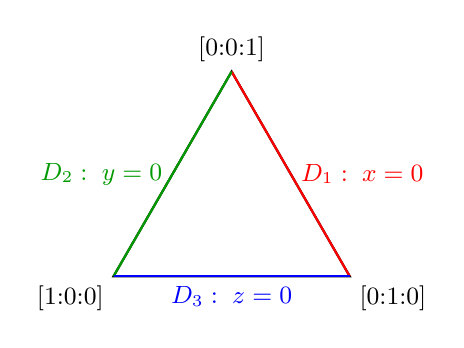
\begin{tikzpicture}[scale=1.0, every node/.style={font=\small}]
        \coordinate (A) at (0,0);
        \coordinate (B) at (3,0);
        \coordinate (C) at (1.5,2.6);

        % triangle representing the projective plane
        \draw[thick] (A) -- (B) -- (C) -- cycle;

        % coordinate lines (toric boundary)
        \draw[thick, red] (B) -- (C) node[midway, right] {\(D_1:\;x=0\)};
        \draw[thick, green!60!black] (A) -- (C) node[midway, left] {\(D_2:\;y=0\)};
        \draw[thick, blue] (A) -- (B) node[midway, below] {\(D_3:\;z=0\)};

        % vertices (torus-fixed points)
        \node[below left] at (A) {[1:0:0]};
        \node[below right] at (B) {[0:1:0]};
        \node[above] at (C) {[0:0:1]};
    \end{tikzpicture}
    \end{center}
\end{frame}


\begin{frame}[c]{Further questions}

    Here are two further questions we are interested in:

    \begin{itemize}
        \item generalize the case \(\rho(Y)=1\) (hence \(\rho(X)=2\)) to any \(X\) with picard number \(2\);
        \item study the decomposition of cones with the decomposition of \(K_X\) and \(R_f\) and use them to study the case \(R_f\) is big.
    \end{itemize}
    
\end{frame}


% ----------------------------------------------------------

% Thank you slide
{
    \setbeamertemplate{background}{}
    \begin{frame}[plain]

    \vspace{0.2\textheight}
    \Huge{\centerline{\textbf{\alert{Thank You!}}}}

    \vfill
    \centerline{\includegraphics[width=0.35\textwidth]{\ECNULibThanks}}
    \end{frame}
}


\end{document}